\documentclass[11pt]{article}
\usepackage[margin=24mm]{geometry}
\usepackage{amsmath,amssymb}
\usepackage{tikz}\usetikzlibrary{positioning,arrows.meta,decorations.pathreplacing}
\begin{document}
\section{Flowchart}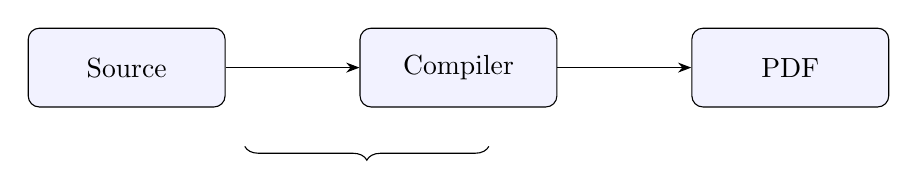
\begin{tikzpicture}[node distance=17mm,box/.style={draw,rounded corners,fill=blue!5,minimum width=25mm,minimum height=10mm},>=Stealth]\node[box](a){Source};\node[box,right=of a](b){Compiler};\node[box,right=of b](c){PDF};\draw[->](a)--(b);\draw[->](b)--(c);\draw[decorate,decoration={brace,amplitude=5pt}] (4.6,-1)--(1.5,-1);\end{tikzpicture}
\end{document}
